 La Unión Internacional de Telecomunicaciones (UIT) \cite{video-encoding-definition} define el proceso de codificación de vídeo como el proceso de transformar una secuencia de imágenes de vídeo de entrada en una representación digital codificada conforme a un estándar, para facilitar su almacenamiento, transmisión y posterior decodificación o reproducción. En este conjunto de bits, también se encuentra codificado el audio e información de interés para los codificadores, lo cual es necesario para llevar a cabo diversos procesos como la transcodificación o la decodificación. 

 El conjunto de pasos y técnicas empleado para llevar a cabo la codificación y decodificación de video se encuentra definido en estándares, los cuyo funcionamiento es establecido por las organizaciones Moving Picture Expert Group (MPEG) y la Unión Internacional de Telecomunicaciones (ITU), y el conjunto de empresasas que confroman el Alliance for Open Media (AOM) \footnote{\url{https://aomedia.org/about/members/}}. Cada uno de los estandares de codificación es diseñado de tal forma que logra satisfacer las necesidad de calidad y de consumo con tenido, asi superar las limitaciones que el estandar actual no es capaz de alcanzar.

 Empleando como base el estándar definido, se llevan a cabo múltiples implementaciones conocidas como codificadores o codecs, los cuales llevan a cabo el proceso de codificación/decodificación de video. Cada uno de estos códecs se diferencia del resto de códecs de una misma generación en base a múltiples atributos y cuestiones técnicas, como el hardware que lleva a cabo la codificación (CPU o CPU + GPU) hasta el bit de color empleado. No obstante, todos ellos mantienen una serie de características comunes e invariables, debido a que la estandarización de procesos fue ideada para lograr un marco común de trabajo a través del cual la industria pudiera adaptarse y atender la demanda de consumo de contenido de la forma correspondiente. 

\subsection{Estandares de Codificación}
 En base a la encuenta realizada por \textit{Bitmovin} \cite{bitmovin-9-report}, los estandares mas utilizados en la actualidada son \textbf{H.264/AVC}, con un \textit{$65\%$}, y \textbf{H.265/HEVC}, con una cuota de uso del \textit{$41\%$}. Seguidos \textbf{AV1} con un \textit{16\%}, \textbf{VP9} con un \textit{13\%} y \textbf{H.266/VCC} con un \textit{6\%}, repartiendo el porcentaje restante a los estandares \textit{MPEG-5/EVC, MPEG-5/LC-EVC y VP8}. 

 En cuanto al estandar \textit{H.264/AVC}, salio al mercado en el año 2003 y fue desarrollado por el MPEG con el fin de introduccion mejoras significativas respecto a estándares anteriores como MPEG-2, H.263 y MPEG-4 Part 2. Introdujo técnicas más avanzadas de predicción, transformada y codificación entrópica logrando alcanzar una calidad de vídeo perceptualmente equivalente utilizando aproximadamente entre un tercio y la mitad de la tasa de bits requerida por MPEG-2. Entre sus principales características destacan el uso de tamaños de bloque variables, múltiples imágenes de referencia, predicción de movimiento con precisión de cuarto de píxel y los métodos de codificación entrópica CAVLC y CABAC, que contribuyen a mejorar la eficiencia de compresión. Además, su flexibilidad permitió su aplicación en un amplio rango de escenarios, desde servicios de vídeo de bajo bitrate hasta contenidos de alta definición y transmisión de contenido a traves de la web via IP \cite{h264-survery}.

 Sin embargo, estas mejoras implicaron un aumento de la complejidad computacional, especialmente durante la codificación, constituyendo una de sus principales desventajas y estableciendo un compromiso entre eficiencia de compresión y recursos necesarios para su procesamiento. Por este motivo, se desarrollo el estandar \textit{H.265/HEVC} como una evolución de H.264/AVC con el objetivo de reducir aproximadamente un $50\%$ la tasa de bits necesaria para alcanzar una calidad de vídeo equivalente. Para ello, mantiene la arquitectura de codificación híbrida de su predecesor, pero introduce mejoras en prácticamente todas las etapas del proceso de codificación. Lo que ha resultado en una mayor compresion de video, con una mayor calidad y una mayor tasa de bits. Como resultado, \textit{H.265} presenta una carga computacion superior a \textit{H.264} que se traduce en un mayor tiempo de computacion y un mayor consumo de recursos, como se muestra en el articulo \textit{Towards H.265 video coding standard} \cite{h265-survery}. 

 Con el objetivo de continuar mejorando la eficiencia de compresión de \textit{H.264} y \textit{H.265}, así como de dar respuesta a las nuevas necesidades de distribución y consumo de vídeo, especialmente ante el incremento de resoluciones como UHD y 8K y la aparición de nuevos escenarios como el vídeo en 360º, la realidad virtual y el \textit{streaming} desde dispositivos móviles, se desarrollaron nuevos estándares de codificación. Por un lado, la Alliance for Open Media (AOM) desarrolló \textit{AV1}, publicado en 2018, como un estándar abierto y libre de royalties, orientado principalmente a la distribución de vídeo a través de Internet y que proporciona una mejora significativa de la eficiencia de compresión respecto a H.264 y H.265. Por otro lado, MPEG y VCEG, a través del Joint Video Experts Team (JVET), desarrollaron el estándar \textit{Versatile Video Coding (VVC)}, publicado en 2020, cuyo objetivo fue alcanzar una reducción de aproximadamente el $50\%$ de la tasa de bits respecto a \textit{HEVC} manteniendo una calidad equivalente. De forma paralela, MPEG desarrolló \textit{Essential Video Coding (EVC)}, planteado como una alternativa que busca mejorar la eficiencia de H.264 y H.265 manteniendo un equilibrio entre eficiencia, complejidad y condiciones de licenciamiento. Estos estándares representan una nueva generación de codecs que buscan incrementar la eficiencia de compresión y adaptarse a las nuevas demandas de consumo de vídeo, aunque con diferentes compromisos en términos de complejidad computacional, eficiencia y licenciamiento \cite{codecs-landscape}.

 En cuanto al desarrollo de este TFM, se han seleccionado dos implementaciones por cada uno de los estándares \textit{H.264} y \textit{H.265}. Dos de las implementaciones de código basadas en CPU (\textit{libx264} y \textit{libx265}) y las otras dos restantes basadas en aceleración mediante GPU (\textit{h264\_nvenc} y \textit{hevc\_nvenc}). Para llevar a cabo los procesos de codificación, se empleará la herramienta FFMPEG, ampliamente utilizada en la industria y que además cuenta con las cuatro implementaciones. 

 \begin{figure}[H]
     \centering
     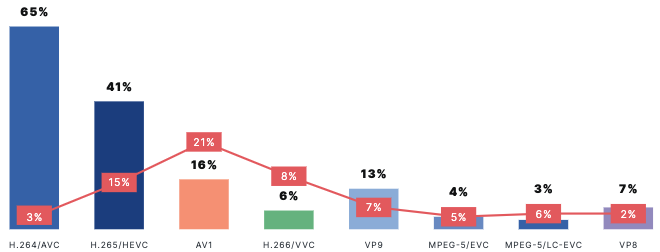
\includegraphics[width=\linewidth]{figs/arte/codec-survery-indutry.png}
     \caption{Estandares de codificacion empleados en produccion frente a futura tasa de implementacion(linea roja), encuenta llevada a cabo por Bitmovin \cite{bitmovin-9-report}}
     \label{fig:codec-implementation-bitmovin}
 \end{figure}
 
\subsection{Paralelización y utilización de threads}



\subsection{Proceso de Codificación}
 La arquitectura general del proceso de codificación es similar tanto en \textit{H.264} como en \textit{H.265}, ya que ambos estándares se basan en la arquitecura \textit{Hybrid Block-Base}, descrita en el articlo \textit{THE VIDEO CODEC LANDSCAPE IN 2020}. A continuación, se describen las principales etapas que intervienen en el proceso de codificación de vídeo, tomando como referencia el trabajo \textbf{Engineering and Technology Quarterly Reviews} \cite{h264-vs-h265}, junto con la documentación oficial de la \textit{International Telecommunication Union (ITU)} correspondiente a los estándares \textit{H.264} \cite{itu-official-h264} y \textit{H.265} \cite{itu-official-h265}.
 
 \begin{enumerate} 
  \item \texttt{Acondicionamiento y submuestreo de color:} 
  En primer lugar, la información de color del vídeo puede convertirse desde el modelo RGB a un espacio de color como YUV, en el que se separan las componentes de luminancia y crominancia. Esta separación permite aplicar diferentes niveles de resolución a cada componente mediante técnicas de submuestreo de crominancia, reduciendo la cantidad de información necesaria para representar el vídeo sin producir una pérdida visual significativa. Los principales esquemas de submuestreo utilizados se recogen en la tabla \ref{tab:croma-yub-esquema}.
 
  \item \texttt{Particionado de los fotogramas:} 
  Una vez realizado el acondicionamiento de la información, cada fotograma se divide en diferentes unidades que serán procesadas de forma independiente. En \textit{H.264}, la unidad básica de procesamiento es el \textit{macroblock}, que presenta un tamaño máximo de 16$\times$16 muestras de luminancia y puede dividirse en particiones de menor tamaño para realizar las operaciones de predicción y transformación.

  Por su parte, \textit{H.265} sustituye este mecanismo por una estructura jerárquica basada en las \textit{Coding Tree Units} (CTU), que pueden alcanzar tamaños de hasta 64$\times$64 muestras y dividirse posteriormente en diferentes \textit{Coding Units} (CU), \textit{Prediction Units} (PU) y \textit{Transform Units} (TU). Esta estructura proporciona una mayor flexibilidad a la hora de adaptar el tamaño de las unidades a las características del contenido.
 
  \item \texttt{Predicción espacial y temporal:} 
  Sobre las unidades obtenidas se lleva a cabo un proceso de predicción destinado a reducir la redundancia presente en el vídeo. En la predicción \textit{intra-frame}, también denominada predicción espacial, se utiliza información procedente de bloques vecinos pertenecientes al mismo fotograma para estimar el contenido del bloque actual. Por otro lado, la predicción \textit{inter-frame}, o predicción temporal, utiliza información procedente de otros fotogramas de referencia. Para ello se calculan vectores de movimiento que permiten identificar las diferencias entre el bloque actual y su correspondiente región en los fotogramas de referencia.
 
  En función del mecanismo de predicción empleado, los fotogramas de una secuencia pueden clasificarse principalmente como \textit{I}, \textit{P} o \textit{B}. Los fotogramas \textit{I} se codifican utilizando únicamente información del propio fotograma, mientras que los fotogramas \textit{P} y \textit{B} utilizan información de otros fotogramas de referencia. Los fotogramas \textit{B} pueden utilizar referencias tanto anteriores como posteriores dentro de la secuencia.
 
  Durante la selección de determinadas decisiones de codificación pueden emplearse técnicas de optimización tasa-distorsión. Una formulación habitual es la función:
 
  \begin{equation}
   J = D + \lambda R
  \end{equation}
 
  donde $D$ representa la distorsión introducida, $R$ la tasa de bits necesaria para representar la información y $\lambda$ el multiplicador de Lagrange utilizado para establecer el equilibrio entre ambos factores.
 
  \item \texttt{Transformación y cuantización:} Una vez realizada la predicción, la información residual resultante se transforma al dominio de la frecuencia mediante transformaciones matemáticas basadas principalmente en la \textit{Discrete Cosine Transform} (DCT). Esta transformación permite representar la información mediante diferentes componentes frecuenciales, facilitando la posterior eliminación de aquellas que presentan una menor relevancia. 

  En \textit{H.264} se utilizan principalmente transformaciones con tamaños de 4$\times$4 y 8$\times$8, mientras que \textit{H.265} amplía los tamaños disponibles hasta 32$\times$32. Además, \textit{H.265} incorpora una transformación basada en la \textit{Discrete Sine Transform} (DST) para determinados bloques intra de luminancia. Posteriormente, los coeficientes obtenidos son cuantizados, reduciendo la precisión de determinados componentes y permitiendo disminuir la cantidad de información necesaria para representar el vídeo.
 
  \item \texttt{Filtrado:} Como consecuencia de la codificación por bloques pueden aparecer determinados artefactos visuales en las zonas de transición entre bloques. Para reducir estos efectos, \textit{H.264} incorpora un filtro de desbloqueo (\textit{Deblocking Filter}). \textit{H.265} mantiene este mecanismo e incorpora además el \textit{Sample Adaptive Offset} (SAO), que permite realizar un procesamiento adicional de los valores reconstruidos con el objetivo de mejorar la calidad de la imagen.
 
  \item \texttt{Codificación entrópica:} Finalmente, los datos resultantes del proceso de transformación, cuantización y predicción son sometidos a una codificación entrópica con el objetivo de reducir aún más la cantidad de bits necesarios para representar la información. \textit{H.264} permite utilizar técnicas como \textit{CAVLC} (\textit{Context-Adaptive Variable-Length Coding}) y \textit{CABAC} (\textit{Context-Adaptive Binary Arithmetic Coding}), mientras que \textit{H.265} utiliza \textit{CABAC} como mecanismo de codificación entrópica.
 \end{enumerate}

 El conjunto de estas etapas permite obtener un flujo de vídeo codificado que contiene la información necesaria para reconstruir la secuencia original durante el proceso de decodificación. Este flujo puede posteriormente encapsularse junto con otros tipos de información, como el audio, dentro de un formato contenedor como \textit{MP4}, \textit{MKV} o \textit{MPEG-TS}. El proceso de encapsulado no forma parte directamente del estándar de codificación de vídeo, sino que permite organizar y transportar los diferentes flujos que componen el contenido multimedia.
 
 Las diferencias existentes entre \textit{H.264} y \textit{H.265} tienen una repercusión directa sobre los recursos computacionales necesarios para realizar la codificación. En particular, la mayor flexibilidad en el particionado, los mecanismos adicionales de predicción y las nuevas herramientas de procesamiento introducidas por \textit{H.265} permiten mejorar la eficiencia de compresión, pero pueden incrementar la complejidad computacional del proceso respecto a \textit{H.264}. Esta diferencia resulta especialmente relevante en el contexto de este trabajo, donde se analiza cómo el estándar utilizado, las características del contenido y los recursos asignados al proceso de codificación afectan tanto al consumo energético como al tiempo de ejecución.

 \begin{table}[htbp]
 \centering
 \begin{minipage}{0.45\textwidth}
   \centering
   \begin{tabularx}{\linewidth}{|>{\centering\arraybackslash}X|>{\centering\arraybackslash}X|}
     \hline
     \rowcolor[HTML]{C0C0C0} 
     \textbf{Formato} & \textbf{Información de Color Retenida} \\ \hline
     4:4:4 & 100\% \\ \hline
     4:2:2 & 50\%  \\ \hline
     4:2:0 & 25\%  \\ \hline
     4:1:1 & 25\%  \\ \hline
     4:0:0 & 0\%   \\ \hline
   \end{tabularx}
   \caption{Tabla de tipos de submuestreo mediante croma y porcentaje de información de color que retiene.}
   \label{tab:croma-yub-esquema}
 \end{minipage}
 \hfill  
 \begin{minipage}{0.45\textwidth}
   \centering
   \begin{tabularx}{\linewidth}{|>{\centering\arraybackslash}X|>{\centering\arraybackslash}X|}
     \hline
     \rowcolor[HTML]{C0C0C0} 
     \textbf{Tipo de Frame} & \textbf{Compresión} \\ \hline  
     I-Frame (Intra) & Baja \\ \hline
     P-Frame (Predicción) & Media \\ \hline
     B-Frame (Bi-directional) & Alta \\ \hline
   \end{tabularx}
 \caption{Tablas comparativas: (izquierda) submuestreo de croma, (derecha) compresión espaciotemporal.}
 \label{tab:compresion-sp}
 \end{minipage}
 \end{table}
 
 
\subsection{Codificación Acelerada por Hardware}

 Tradicionalmente, los procesos de codificación de vídeo se han ejecutado principalmente sobre la CPU mediante implementaciones software de los distintos estándares de compresión. Sin embargo, el incremento progresivo de la demanda de contenido multimedia de alta resolución y elevada frecuencia de imagen, junto con la generalización de los servicios de vídeo bajo demanda y streaming, ha incrementado considerablemente la carga computacional asociada a estos procesos. Esta evolución ha favorecido la incorporación de mecanismos de aceleración hardware capaces de trasladar parte de las operaciones de codificación desde la CPU hacia unidades de procesamiento especializadas, entre las que destacan las GPU.

 Este incremento de la demanda está relacionado tanto con la evolución de la calidad del contenido, con resoluciones como 4K UHD y frecuencias de hasta 60 o 120 fps, como con el cambio en los patrones de consumo. El contenido multimedia se distribuye actualmente a través de un amplio conjunto de dispositivos, desde ordenadores personales hasta teléfonos móviles, tabletas y Smart TV, y se entrega principalmente mediante plataformas de streaming. Como consecuencia, una parte significativa de la carga computacional asociada al procesamiento y distribución del contenido se concentra en centros de procesamiento de datos (CPD) y redes de distribución de contenido (Content Delivery Networks, CDN), donde el volumen de contenido procesado puede ser considerablemente elevado.
 
 Este aumento de la carga de trabajo asociada a la codificación puede provocar un incremento de los tiempos de procesamiento y de los recursos computacionales necesarios, especialmente cuando se requiere generar diferentes representaciones de un mismo contenido para adaptarlo a distintas resoluciones, tasas de bits y dispositivos de consumo. En estos escenarios, una ejecución basada exclusivamente en CPU puede llegar a convertirse en un factor limitante, generando cuellos de botella y un incremento del consumo de recursos y energía. No obstante, el comportamiento de la CPU no es necesariamente desfavorable en todos los escenarios, ya que su rendimiento puede resultar competitivo cuando se trabaja con contenidos de menor resolución y frecuencia de imagen, donde la carga computacional asociada a la codificación es inferior \cite{gpuvscpu-videoencoding}.
 
 Los resultados obtenidos en el trabajo \cite{tokyo-livestreming-acceleration-gpu} muestran que, en escenarios de streaming UHD, las implementaciones de codificación basadas exclusivamente en CPU pueden presentar un elevado coste computacional y energético, especialmente a medida que aumenta la resolución y la complejidad del contenido. Estos resultados ponen de manifiesto que, en escenarios de elevada carga de trabajo, la utilización de mecanismos de aceleración hardware puede constituir una alternativa para reducir el tiempo necesario para completar la codificación y mejorar la eficiencia del procesamiento.
 
 Por su parte, la utilización de mecanismos de aceleración hardware permite descargar parte de la carga computacional asociada a la codificación de la CPU hacia unidades especializadas de la GPU. En base a los resultados obtenidos en el trabajo \textit{Evaluation of Hardware-based Video Encoders on Modern GPUs for UHD Live-Streaming} \cite{tokyo-livestreming-acceleration-gpu}, se observaron diferencias significativas en el tiempo de codificación y en el consumo energético entre implementaciones software y hardware de determinados estándares. En particular, se identificaron diferencias entre implementaciones de H.265/HEVC como \textit{x265} y \textit{hevc\_nvenc}, mostrando el potencial de la aceleración hardware para reducir el coste computacional asociado a la codificación de vídeo en escenarios de alta resolución y streaming.
 
 No obstante, la utilización de aceleración hardware no implica necesariamente una mejora uniforme para cualquier tipo de contenido o configuración. Los resultados obtenidos en \cite{gpuvscpu-videoencoding} muestran que, para determinadas condiciones de resolución y frecuencia de imagen, las implementaciones basadas en CPU pueden proporcionar resultados competitivos en términos de calidad y tiempo de codificación, sin que la utilización de una implementación acelerada mediante GPU suponga necesariamente una ventaja significativa. Por tanto, la elección entre una implementación basada en CPU o en GPU debe considerar las características del contenido, la resolución, la frecuencia de imagen y las necesidades concretas del escenario de distribución.
 
 También es necesario tener en cuenta la plataforma sobre la que se llevará a cabo el consumo y distribución del contenido, ya que la configuración del bitrate y de los parámetros de codificación puede afectar de diferente forma a la calidad final percibida por el consumidor. Este aspecto resulta especialmente relevante al establecer una relación entre calidad de vídeo, tasa de bits, tiempo de codificación y consumo energético. No obstante, el análisis de la calidad subjetiva de los usuarios y de la adaptación del contenido a las diferentes plataformas queda fuera del alcance de este TFM.
 
 \begin{figure}[H]
     \centering
     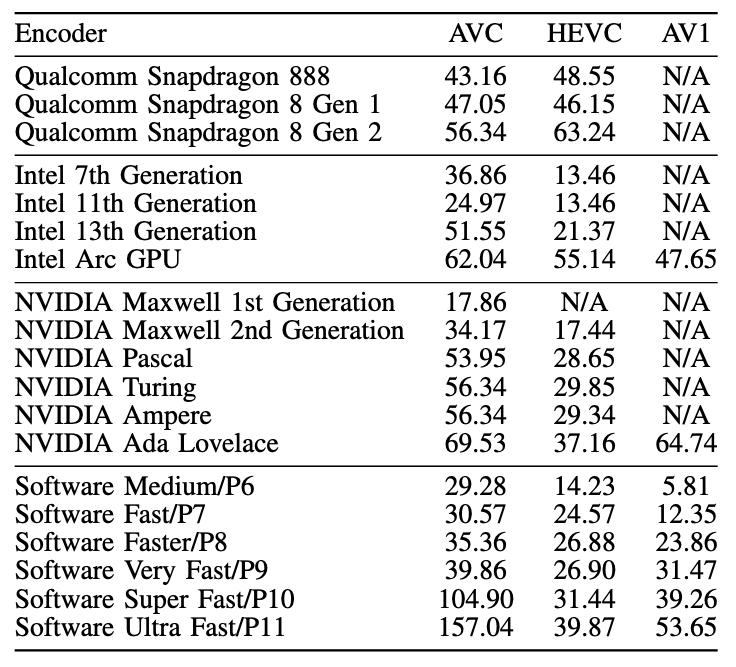
\includegraphics[width=0.4\linewidth]{figs/arte/tokyo-encodign-throughput.png}
     \caption{Frames por segundo de un proceso de codificacion a 2016p/4k que alcanzan a codificar cada una de las arquitecturas del Hardware comparado en el estudio \cite{tokyo-livestreming-acceleration-gpu}}
     \label{fig:tokyo-encoding-throughtput}
 \end{figure}


